\section{问题二：变物性热湿耦合模型}

\subsection{问题分析}

问题二研究药材在变物性条件下的传热与失水特征，重点给出前三小时内各规定位置的温度和干基含水率。问题一给出了预热阶段的传递基准；本问则从题面初值重新积分，不将 $1800\,\mathrm{s}$ 设为边界切换时刻。这样处理可以在同一环境边界下考察状态相关物性随温度和含水率变化所产生的反馈。

附件~1 的烘房温度和有效水分浓度在相邻采样点之间采用分段线性插值，在 $0$--$10800\,\mathrm{s}$ 内形成连续边界。题面未为本问另行给出换热系数和传质系数，故沿用附录~2 的 $h=25\,\mathrm{W/(m^2\cdot K)}$ 和 $h_m=8\times10^{-7}\,\mathrm{m/s}$ 作为缺参条件下的延续假设。{\heiti\bfseries 药材半径固定为 $R=0.02\,\mathrm{m}$，不考虑收缩、潜热、内部对流及额外热湿源项。}

与问题一中热物性取常数而扩散系数仅随含水率变化的设定相比，本问采用附录~3 的状态相关关系。含水率会同时改变密度、比热容和导热系数，温度与含水率共同决定有效扩散系数，因此需要求解温度场和水分场的联立方程。该模型描述的是题面参数下的变物性有效传递过程，不等同于包含蒸发焓的完整能量模型。

\subsection{模型建立}

取 $r\in[0,R]$ 为到圆柱中心轴的径向距离，$T(r,t)$ 以摄氏度表示，$C(r,t)$ 为干基含水率。在扩散系数的指数项中采用绝对温度 $T_K=T+273.15$，其中 $T_K$ 的单位为 K；除该指数项外，方程和边界中的温度均使用摄氏度数值。附录~3 的状态相关物性写为

\begin{equation}
\begin{aligned}
  \rho(C)&=650+128C,\\[2pt]
  c_p(C)&=1450+2736\frac{C}{C+1},\\[2pt]
  k(C)&=0.21+0.38\frac{C}{C+1},\\[2pt]
  D(C,T)&=2.4\times10^{-3}
  \,\mathrm e^{-\frac{0.45}{C}}
  \,\mathrm e^{-\frac{3850}{T_K}}.
\end{aligned}
\label{eq:q2-properties}
\end{equation}

其中 $\rho$、$c_p$、$k$ 和 $D$ 的单位分别为 $\mathrm{kg/m^3}$、$\mathrm{J/(kg\cdot K)}$、$\mathrm{W/(m\cdot K)}$ 和 $\mathrm{m^2/s}$。由能量守恒和 Fick 型有效扩散得到固定半径下的联立方程

\begin{equation}
\left\{
\begin{aligned}
  \rho(C)c_p(C)\frac{\partial T}{\partial t}
  &=\frac{1}{r}\frac{\partial}{\partial r}
    \left(rk(C)\frac{\partial T}{\partial r}\right),\\
  \frac{\partial C}{\partial t}
  &=\frac{1}{r}\frac{\partial}{\partial r}
    \left(rD(C,T)\frac{\partial C}{\partial r}\right),
  \qquad 0<r<R,\ t>0.
\end{aligned}
\right.
\label{eq:q2-pde}
\end{equation}

\Needspace{14\baselineskip}
完整初边值条件为

\begin{equation}
\left\{
\begin{aligned}
  T(r,0)&=28\,{}^\circ\mathrm{C},\\[2pt]
  C(r,0)&=2.55\,\mathrm{kg/kg},\\[2pt]
  \left.\frac{\partial T}{\partial r}\right|_{r=0}&=0,\\[2pt]
  \left.\frac{\partial C}{\partial r}\right|_{r=0}&=0,\\[2pt]
  -k(C_s)\left.\frac{\partial T}{\partial r}\right|_{r=R}
    &=h\,[T_s-T_\infty(t)],\\[2pt]
  -D(C_s,T_s)\left.\frac{\partial C}{\partial r}\right|_{r=R}
    &=h_m\,[C_s-C_\infty(t)].
\end{aligned}
\right.
\label{eq:q2-ibvp}
\end{equation}

其中 $T_s=T(R,t)$、$C_s=C(R,t)$。对附件~1 中的相邻采样时刻 $t_m$、$t_{m+1}$，令

\begin{equation}
  \lambda(t)=\frac{t-t_m}{t_{m+1}-t_m},\qquad
  \begin{aligned}
  T_\infty(t)&=T_{\infty,m}+\lambda(t)(T_{\infty,m+1}-T_{\infty,m}),\\
  C_\infty(t)&=C_{\infty,m}+\lambda(t)(C_{\infty,m+1}-C_{\infty,m}).
  \end{aligned}
  \label{eq:q2-boundary-interpolation}
\end{equation}

\subsection{模型求解}

对径向区域作均匀离散，温度和水分均采用{\heiti\bfseries 守恒通量离散}，使相邻控制体共用同一界面通量；界面物性取相邻节点的算术平均，圆心按轴对称极限处理，表面施加 Robin 交换条件。空间离散后，采用{\heiti\bfseries BDF 自适应积分}求解温度场和水分场的联立非线性系统。

由于原始含水率变量在非线性内部试探中可能产生非正值，积分器内部采用可逆对数坐标 $z_i=\log C_i$，每次评价时由 $C_i=\mathrm e^{z_i}$ 回到物理方程。该变换只改变数值坐标，不改变含水率的物理定义；解析稀疏 Jacobian 保留温度与含水率之间的交叉依赖。

为分辨初期表面附近的含水率变化，逐级加密径向网格，最终采用 $N=10240$ 个径向区间。{\heiti\bfseries 最终计算}采用相对容差 $10^{-10}$、绝对容差 $10^{-12}$ 和最大内部步长 $2.5\,\mathrm{s}$；按题意每隔 $1\,\mathrm{s}$、每隔 $0.1\,\mathrm{cm}$ 输出，得到每个时刻 $21$ 个径向位置的状态值。每秒输出不代表以 $1\,\mathrm{s}$ 为积分步长，内部步长由误差控制自适应确定。

数值检验覆盖全部规定输出点。空间比较中，$N=5120$ 与 $N=10240$ 的最大差异分别为 $e_T=3.426781\times10^{-6}\,{}^\circ\mathrm{C}$ 和 $e_C=3.731918\times10^{-6}\,\mathrm{kg/kg}$；时间设置收紧后的最大差异分别为 $3.751870\times10^{-6}\,{}^\circ\mathrm{C}$ 和 $4.548273\times10^{-8}\,\mathrm{kg/kg}$。两组加密计算所得六个时刻、五个位置的表值在四位小数下保持一致。上述检验说明离散与积分设置在规定输出上的数值变化已受到控制，但不将其等同于端部、潜热等物理简化误差的消除。

\Needspace{16\baselineskip}
\subsection{结果分析}

规定时刻和规定径向位置的温度见表~\ref{tab:q2-temperature}。表中每隔 $0.5\,\mathrm{h}$ 给出一个时刻，数值由计算解在五个径向位置提取并四舍五入到四位小数。

\begin{table}[H]
  \centering
  \fontsize{10.5pt}{12.6pt}\selectfont
  \renewcommand{\arraystretch}{1.25}
  \captionsetup{font=small,labelfont=bf,textfont=bf}
  \caption{3小时内药材的温度}
  \label{tab:q2-temperature}
  \begin{tabularx}{0.92\textwidth}{|>{\centering\arraybackslash}p{0.23\textwidth}|*{5}{>{\centering\arraybackslash}X|}}
    \hline
    \multirow{2}{*}{时间/h} & \multicolumn{5}{|c|}{到药材中心的距离/cm} \\
    \cline{2-6}
     & 0 & 0.5 & 1 & 1.5 & 2 \\
    \hline
    0.5 & 32.1892 & 32.3821 & 32.9659 & 33.9608 & 35.4130 \\
    \hline
    1.0 & 40.3816 & 40.5536 & 41.0605 & 41.8782 & 42.9976 \\
    \hline
    1.5 & 45.8468 & 45.9348 & 46.1930 & 46.6051 & 47.1400 \\
    \hline
    2.0 & 48.4502 & 48.4881 & 48.5984 & 48.7736 & 49.0033 \\
    \hline
    2.5 & 49.4670 & 49.4792 & 49.5136 & 49.5653 & 49.6609 \\
    \hline
    3.0 & 49.8495 & 49.8553 & 49.8746 & 49.9101 & 49.9664 \\
    \hline
  \end{tabularx}
\end{table}


药材温度呈现由表及里的响应滞后。$0.5\,\mathrm{h}$ 时，中心温度为 $32.1892\,{}^\circ\mathrm{C}$，表面温度为 $35.4130\,{}^\circ\mathrm{C}$，两者相差 $3.2238\,{}^\circ\mathrm{C}$；{\heiti\bfseries 到 $3\,\mathrm{h}$ 时，中心和表面温度分别为 $49.8495$ 和 $49.9664\,{}^\circ\mathrm{C}$，温差缩小到 $0.1169\,{}^\circ\mathrm{C}$。}这说明热扩散在前三小时内逐渐减小早期径向温差。

相同时空位置的干基含水率见表~\ref{tab:q2-moisture}。

\begin{table}[H]
  \centering
  \caption{3 小时内药材的干基含水率（$\mathrm{kg/kg}$）}
  \label{tab:q2-moisture}
  \begin{tabular}{rrrrrr}
    \toprule
    时间/h & $0\,\mathrm{cm}$ & $0.5\,\mathrm{cm}$ & $1\,\mathrm{cm}$ & $1.5\,\mathrm{cm}$ & $2\,\mathrm{cm}$ \\
    \midrule
    0.5 & \resultblank{--} & \resultblank{--} & \resultblank{--} & \resultblank{--} & \resultblank{--} \\
    1.0 & \resultblank{--} & \resultblank{--} & \resultblank{--} & \resultblank{--} & \resultblank{--} \\
    1.5 & \resultblank{--} & \resultblank{--} & \resultblank{--} & \resultblank{--} & \resultblank{--} \\
    2.0 & \resultblank{--} & \resultblank{--} & \resultblank{--} & \resultblank{--} & \resultblank{--} \\
    2.5 & \resultblank{--} & \resultblank{--} & \resultblank{--} & \resultblank{--} & \resultblank{--} \\
    3.0 & \resultblank{--} & \resultblank{--} & \resultblank{--} & \resultblank{--} & \resultblank{--} \\
    \bottomrule
  \end{tabular}
\end{table}



水分梯度比温度梯度保持得更久。{\heiti\bfseries $3\,\mathrm{h}$ 时，中心含水率为 $1.7662\,\mathrm{kg/kg}$，表面含水率为 $1.0081\,\mathrm{kg/kg}$，径向差为 $0.7581\,\mathrm{kg/kg}$。}相对于初始值，中心和表面含水率分别下降约 $30.74\%$ 和 $60.47\%$，表明表面已明显失水而中心仍较湿，平均含水率或表面值不能替代全域状态。

为比较空间分布与时间响应，图~\ref{fig:q2-fields} 给出温度和含水率的径向剖面及代表位置的时间曲线。

\begin{figure}[H]
  \centering
  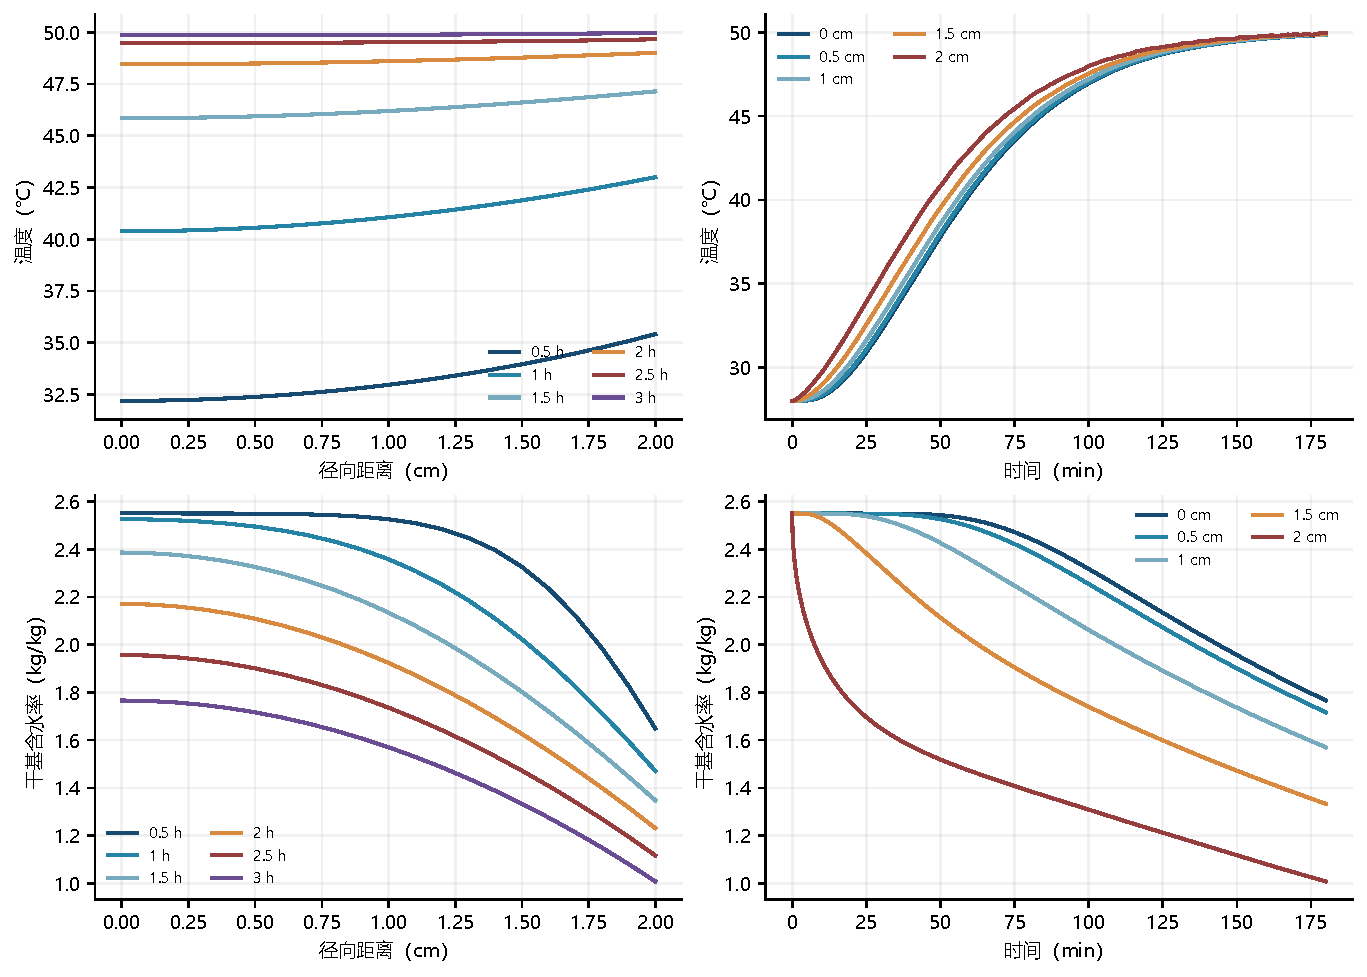
\includegraphics[width=\textwidth]{figures/q2_fields.pdf}
  \caption{问题二温度与干基含水率的径向剖面及时间演化。左列为 $0.5$、$1$、$1.5$、$2$、$2.5$、$3\,\mathrm{h}$ 六个时刻的径向剖面，右列为 $0$、$0.5$、$1$、$1.5$、$2\,\mathrm{cm}$ 五个位置的时间曲线。}
  \label{fig:q2-fields}
\end{figure}

图~\ref{fig:q2-fields} 显示，温度剖面先由表面向内推进，含水率剖面则始终表现为由中心向表面递减的梯度。扩散系数中的温度因子随 $T$ 增大而提高局部 $D$，而含水率降低会使 $\mathrm e^{-\frac{0.45}{C}}$ 变小；两种状态作用共同决定表层与内部之间的水分迁移。初始状态下 $D=5.642\times10^{-9}\,\mathrm{m^2/s}$，$3\,\mathrm{h}$ 时中心和表面的局部值约为 $1.239\times10^{-8}$ 和 $1.027\times10^{-8}\,\mathrm{m^2/s}$。这些数值反映的是状态相关的有效扩散系数，不能单独推出整个药材的水分迁移速率必然加快或减慢。

为展示温度场和含水率场在整个计算窗口内的时空演化，图~\ref{fig:q2-spacetime} 给出 $0$--$3\,\mathrm{h}$、$0$--$2\,\mathrm{cm}$ 范围内的两幅时空曲面。温度曲面随时间整体升高，后期沿径向逐渐趋平；含水率曲面在初期靠近表面处下降较快，内部仍保持较高含水率，随后失水区域向中心推进，至 $3\,\mathrm{h}$ 仍保留明显的径向差异。

\begin{figure}[H]
  \centering
  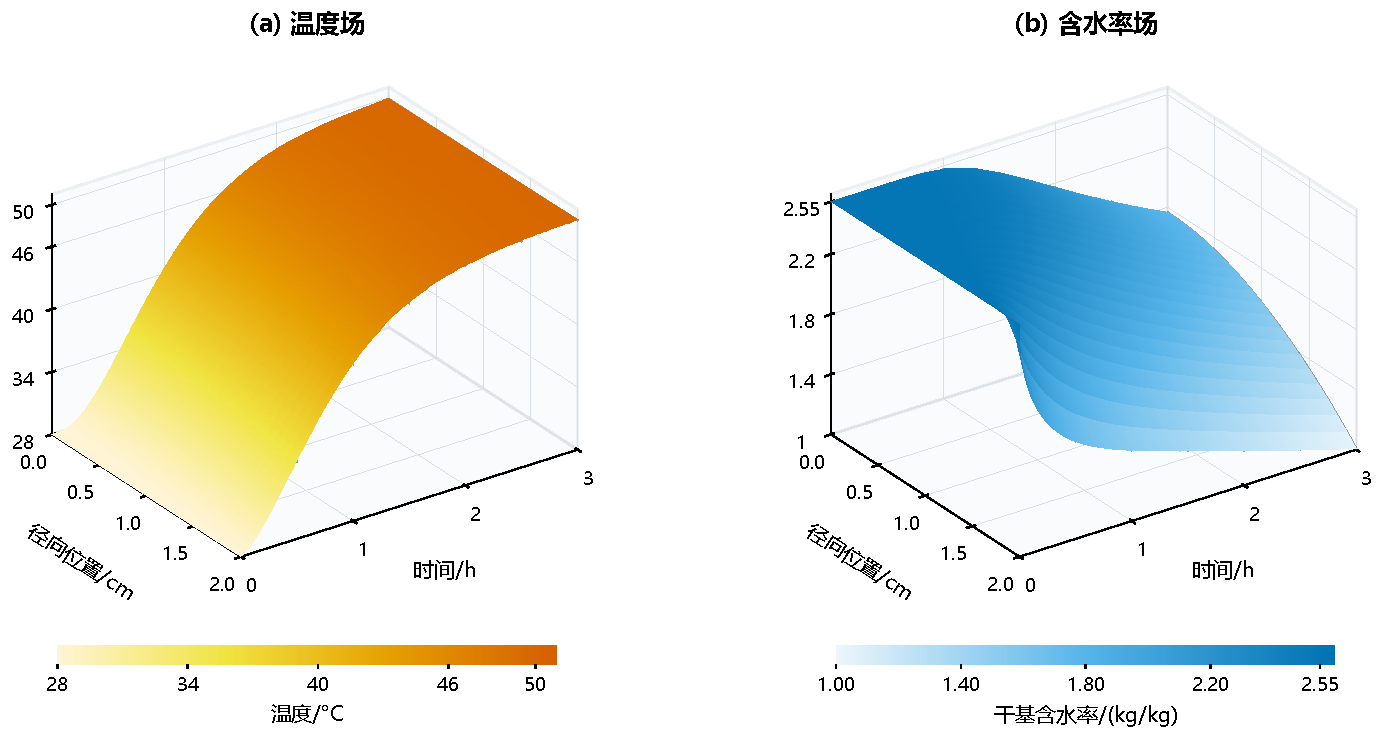
\includegraphics[width=\textwidth]{figures/q2_spacetime.pdf}
  \caption{问题二温度场与干基含水率场的时空演化曲面。横轴为时间，纵轴为径向位置，时间范围为 $0$--$3\,\mathrm{h}$，径向范围为 $0$--$2\,\mathrm{cm}$。}
  \label{fig:q2-spacetime}
\end{figure}

为考察表面交换系数对结果的影响，$h_m$ 降低 $20\%$ 时，$3\,\mathrm{h}$ 时中心和表面含水率相对基准分别增加约 $5.21\%$ 和 $16.80\%$；提高 $20\%$ 时，分别减少约 $4.20\%$ 和 $13.34\%$。$h$ 降低 $20\%$ 时，中心和表面含水率分别增加约 $0.59\%$ 和 $0.15\%$；提高 $20\%$ 时，分别减少约 $0.37\%$ 和 $0.14\%$。在所考察的扰动范围内，含水率对传质系数的变化更为敏感。

为检验上述结果与问题一的衔接，在共同初值、边界、半径以及 $0$--$1800\,\mathrm{s}$ 时间范围内进行逐点比较。问题一在 $1800\,\mathrm{s}$ 时中心和表面温度分别为 $33.5753$ 和 $36.7856\,{}^\circ\mathrm{C}$，问题二分别为 $32.1892$ 和 $35.4130\,{}^\circ\mathrm{C}$，对应低 $1.3861$ 和 $1.3725\,{}^\circ\mathrm{C}$。在水分场，表面含水率由问题一的 $1.5102\,\mathrm{kg/kg}$ 变为问题二的 $1.6486\,\mathrm{kg/kg}$，而 $r=1.5\,\mathrm{cm}$ 处由 $2.3755\,\mathrm{kg/kg}$ 变为 $2.3257\,\mathrm{kg/kg}$。两个模型均表现为表面先升温、失水，中心响应滞后，给出一致的定性趋势。

这种差异与初始物性尺度相符：问题一的体积热容为 $2.132\times10^{6}\,\mathrm{J/(m^3\cdot K)}$、热扩散率为 $1.6886\times10^{-7}\,\mathrm{m^2/s}$，问题二分别为 $3.334695\times10^{6}\,\mathrm{J/(m^3\cdot K)}$ 和 $1.4483\times10^{-7}\,\mathrm{m^2/s}$，初始升温响应因而更具热惯性；初始扩散系数则分别为 $4.9377\times10^{-9}$ 和 $5.6417\times10^{-9}\,\mathrm{m^2/s}$。两问采用不同本构关系，故该对照用于解释预测差异，而不作为精度优劣的判据。{\heiti\bfseries 问题二更适合描述持续升温、失水过程中局部物性反馈的影响。}

% Keep the following question heading together with its opening analysis.
\par\Needspace{9\baselineskip}
